\subsubsection{Тиристор и его свойства}

Тиристор представляет собой четырёхслойную структуру p-n-p-n. Вольтамперная характеристика имеет участок отрицательного сопротивления. 

Тиристор и его ВАХ:
\begin{center}
	\begin{figure}[h!]
		\center{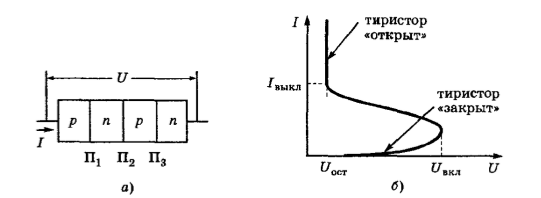
\includegraphics[scale=0.7]{Tir_and_VAH.png}}
		\caption{}	
	\end{figure}
\end{center}

Тиристор можно представить двухтранзисторной моделью:
\begin{center}
	\begin{figure}[h!]
		\center{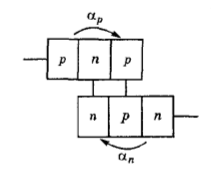
\includegraphics[scale=0.7]{Tir2T.png}}
		\caption{}	
	\end{figure}
\end{center}


Обозначим коэффициент усиления p-n-p транзистора $\alpha_p$, а n-p-n транзистора $\alpha_n$. Ток центрального перехода тиристора П$_2$ складывается из токов коллекторов p-n-p и n-p-n. 

<<<<<<< HEAD
Область p$_1$, в которую попадает ток из внешней цепи , называют анодом, область n$_2$  - катодом, области n$_1$, p$_2$ - базами. если к аноду p$_1$ подключить плюс источника напряжения, а к катоду n$_2$ минус то переходы П$_1$ (между р$_1$ и n$_1$) и  П$_3$ (между р$_2$ и n$_2$) окажутся открытыми, а переход П$_2$ - закрытым (Коллекторный переход). Коллекторный переход смещен в обратном направлении => все приложенное напряжение падает на нем. Ток коллекторного перехода определяет ток во внешней цепи и зависит от потока дырок $\alpha_1$I из эмиттера транзистора типа p-n-p, а также отобратного тока p-n-перехода. Переходы П$_1$ и П$_3$ смещены в прямом направлении, из них в области баз инжектируются носители заряда: дырки - из области р$_1$, электроны - из области n$_2$. Эти носители под действием поля перебрасываются через коллекторный переход. Дырки, инжектированные из области p$_1$ и электроны из n$_2$ движутся через переход П$_2$-коллекторный в противоположных направлениях, создавая общий ток I. Есои внешнее напряжение мало, то оно все падает на коллекторном переходе, ток в цепи мал и равен I$_K0$. Далее с увеличением напряжения (согласно ВАХ) рост тока незначителен, при этом всю большую роль начинают играть носители заряда, образовавшиеся в следствие ударной ионизации, и наступает момент, когда их количество становится настолько большим, что при столкновении с атомами в области p-n перехода они вызывают лавинное размножение носителей. Ток через коллекторный переход увеличивается, его сопротивление падает => растет напряжение на П$_1$ и П$_3$, а также увеличивается инжекция через них. Носители,появившиеся вследствие инжеккции и лавинного размножения, приводят к уменьшению сопротивления всех областей тиристора, и общее падение напряжения на нем становится незначительным - участок с отрицательным дифференциальным сопротивлением на ВАХ.

Рассмотрим схему изображенную на рисунке(с источником и резистором). Если ток во внешней цепи равен I, тогда токи коллекторов:
$I_{K2} = \alpha_2I+I_{{Kb0}_2}$; $I_{K1} = \alpha_1I+I_{{Kb0}_1}$;
здесь $I_{{Kb0}_1}$ и $I_{{Kb0}_2}$ - обратные токи коллекторных переходов каждого из транзисторов, $\alpha_1$, $\alpha_2$ - коэффициенты передачи эмиттерного тока. $I = I_{K1}+I_{K2}$, тогда  $I = \alpha_2I+I_{{Kb0}_2} + \alpha_1I+I_{{Kb0}_1}$.
Пусть M - коэффициент лавинного умножения, тогда $I = M( (\alpha_2 + \alpha_1)I+I_{{Kb0}_2} + I_{{kb0}_1}) = MI_{k0}/(1-M\alpha) $, где $\alpha = \alpha_1+\alpha_2$. Переключение тиристора наступает, когда $M\alpha = 1$. В этом случае ток I ограничен сопротивлением R внешней цепи, а собственное сопротивление тиристора мало.Выключение тиристора осуществляется засчет уменьшения напряжения внешнего истоника до знаечния, при котором ток $I=U/R < I_{off}$.
=======
Область p$_1$, в которую попадает ток из внешней цепи , называют анодом, область n$_2$  - катодом, области n$_1$, p$_2$ - базами. если к аноду p$_1$ подключить плюс источника напряжения, а к катоду n$_2$ минус то переходы П$_1$ (между р$_1$ и n$_1$) и  П$_3$ (между р$_2$ и n$_2$) окажутся открытыми, а переход П$_2$ - закрытым (Коллекторный переход). Коллекторный переход смещен в обратном направлении => все приложенное напряжение падает на нем. Ток коллекторного перехода определяет ток во внешней цепи и зависит от потока дырок $\alpha_1$I из эмиттера транзистора типа p-n-p, а также от обратного тока p-n-перехода. Переходы П$_1$ и П$_3$ смещены в прямом направлении, из них в области баз инжектируются носители заряда: дырки - из области р$_1$, электроны - из области n$_2$. Эти носители под действием поля перебрасываются через коллекторный переход. Дырки, инжектированные из области p$_1$ и электроны из n$_2$ движутся через переход П$_2$-коллекторный в противоположных направлениях, создавая общий ток I. Если внешнее напряжение мало, то оно все падает на коллекторном переходе, ток в цепи мал и равен I$_{K0}$. Далее с увеличением напряжения (согласно ВАХ) рост тока незначителен, при этом всю большую роль начинают играть носители заряда, образовавшиеся в следствие ударной ионизации, и наступает момент, когда их количество становится настолько большим, что при столкновении с атомами в области p-n перехода они вызывают лавинное размножение носителей. Ток через коллекторный переход увеличивается, его сопротивление падает => растет напряжение на П$_1$ и П$_3$, а также увеличивается инжекция через них. Носители,появившиеся вследствие инжекции и лавинного размножения, приводят к уменьшению сопротивления всех областей тиристора, и общее падение напряжения на нем становится незначительным - участок с отрицательным дифференциальным сопротивлением на ВАХ.

Рассмотрим схему изображенную на рисунке(с источником и резистором). Если ток во внешней цепи равен I, тогда токи коллекторов:
$I_{K2} = \alpha_2I+I_{Kb02}$; $I_{K1} = \alpha_1I+I_{Kb01}$;
здесь $I_{Kb01}$ и $I_{Kb02}$ - обратные токи коллекторных переходов каждого из транзисторов, $\alpha_1$, $\alpha_2$ - коэффициенты передачи эмиттерного тока. $I = I_{K1}+I_{K2}$, тогда  $I = \alpha_2I+I_{Kb02}+\alpha_1I+I_{Kb01}$.
Пусть M - коэффициент лавинного умножения, тогда $I = M( (\alpha_2+\alpha_1)I+I_{Kb02}+I_{kb01}) = MI_{k0}/(1-M\alpha) $, где $\alpha = \alpha_1+\alpha_2$. Переключение тиристора наступает, когда $M\alpha = 1$. В этом случае ток I ограничен сопротивлением R внешней цепи, а собственное сопротивление тиристора мало.Выключение тиристора осуществляется за счет уменьшения напряжения внешнего источника до значения, при котором ток $I=U/R < I_{off}$.
>>>>>>> 890bebc60a7e769a8137af80241a9f2afe56e63a

Ток выключения $I_{off}$ соответствует условию $\alpha_pI + \alpha_nI = 1$.

Если в область базы n-p-n транзистора втекает внешний управляющий ток, то условие равенства суммы коэффициентов передачи единице выполняется при меньших токах во внешней цепи => меньше напряжение включения. Это называется уже кремниевым управляемым вентилем. Вольтамперные характеристики:

\begin{center}
	\begin{figure}[h!]
		\center{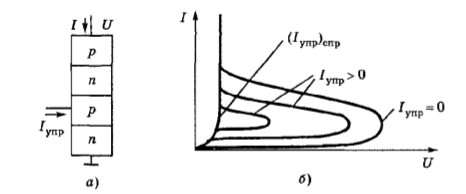
\includegraphics[scale=0.7]{tirI.png}}
		\caption{}	
	\end{figure}
\end{center}

Работа тиристора:
\begin{center}
	\begin{figure}[h!]
		\center{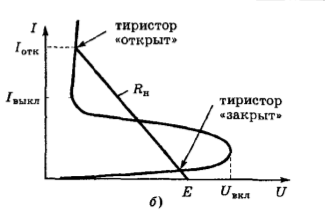
\includegraphics[scale=0.7]{tirworking.png}}
		\caption{}	
	\end{figure}
\end{center}

Рассмотрим включение тиристора в цепь с источником напряжения и нагрузкой R. Предположим, что линия нагрузки пересекает ВАХ тиристора в трёх точках. В закрытом состоянии на тиристоре падает напряжение питания E, так как ток через него очень мал. Переход из закрытого в открытое состояние может произойти вследствие подачи управляющего импульса. Тогда тиристор откроется и останется в состоянии "открыто".

Так как переходы П$_1$ и П$_3$ смещены в прямом направлении, из них в области баз инжектируются носители заряда: дырки из области $p_1$ и  из области $n_2$. Эти носители заряда, диффундируя в областях баз, приближаются к коллекторному переходу и его полем перебрасываются через p-n переход. Дырки, инжектированные из $p_1$ и электроны из $n_2$ движутся через П2 в противоположных направлениях, создавая общий ток I.

При малых значениях внешнего напряжения всё оно практически падает на переходе П2. Поэтому к переходам П1 и П3, имеющим малое сопротивление, приложена маленькая разность потенциалов и диффузия невелика. В этом случае ток через переход равен приблизительно $I_{k0}$. 

Таким образом, свойствами тиристора являются:
\begin{itemize}
\item падение напряжения около 1 В в открытом состоянии. При этом ток может достигать кА.
\item скачкообразный переход по ВАХ
\item $t_{on} << t_{off}$ Обусловлено тем, что заряды, накопившиеся в коллекторе, убираются за счёт рекомбинации в простых тиристорах. Если КУВ => ток управляющий может еще помогать с этой задачей.(источник не указан)
\item имеет участок с отрицательным дифференциальным сопротивлением.

\end{itemize}

Тиристор позволяет использовать часть подаваемой мощности. Тиристорный ключ может проводить в 1 направлении, а в закрытом состоянии способен выдерживать большое прямое и обратное напряжение. 
\begin{center}
	\begin{figure}[h!]
		\center{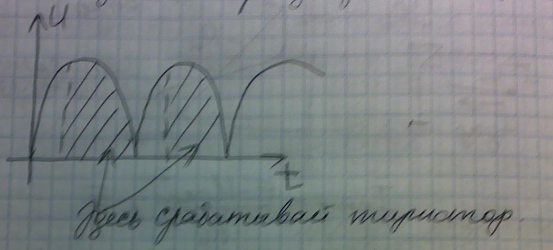
\includegraphics[scale=0.7]{TirLamp}}
		\caption{}	
	\end{figure}
\end{center}

Здесь видно, что тиристор срабатывает на определенном значении входного напряжения. Но выключается не сразу, требуется время $t_{off}$, чтобы он избавился от накопившегося заряда. Поэтому не сразу он переходит в закрытый режим.
